\section{Experimento BRDF duer}

As equações que descrevem esse experimento se encontram em \autoref{fig-duer-eqlang-latex}. O código fonte de entrada para o compilador está dividido em duas partes, parte 1 está no \autoref{cod-duer-eqlang} e a segunda parte está em \autoref{cod-duer-eqlang-pt2}. A renderização dos objetos 3D usando essa BRDF se encontra em \autoref{fig-duer-eqlang}.

%%%%%%%%%%%%%%%%%%%%%%%%%%%%%%%%%%%%%%%%%%%%%%%%%
\subsection{Representação em documento \LaTeX{}}
%%%%%%%%%%%%%%%%%%%%%%%%%%%%%%%%%%%%%%%%%%%%%%%%%
\begin{figure}[H]
    \caption{\label{fig-duer-eqlang-latex} \small Equações da BRDF do experimento duer em documento \LaTeX{}.}
    \begin{center}
        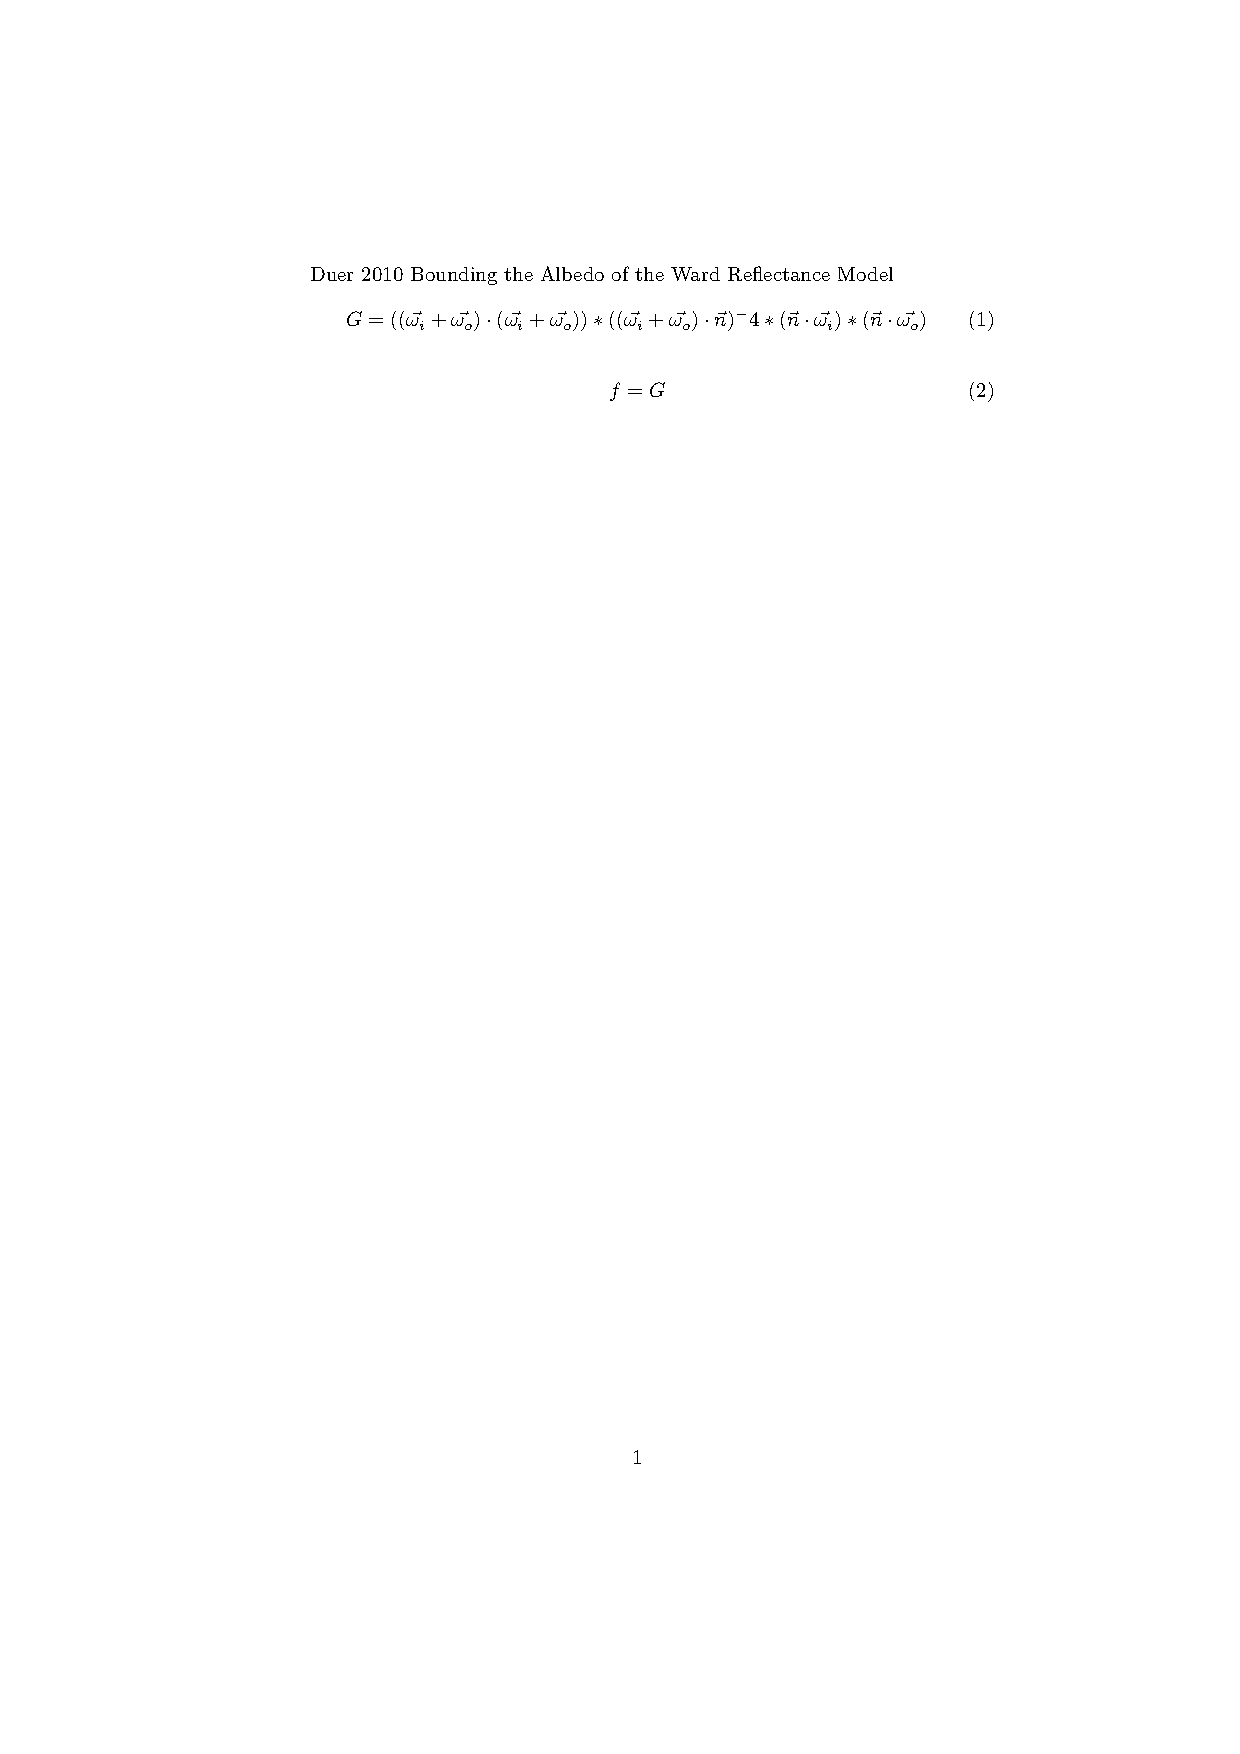
\includegraphics[scale=0.92]{./Imagens/brdfs/duer.pdf}
    \end{center}
\end{figure}

%%%%%%%%%%%%%%%%%%%%%%%%%%%%%%%%%%%%%%%%%%%%%%%%%
\subsection{Visualização do Resultado}
%%%%%%%%%%%%%%%%%%%%%%%%%%%%%%%%%%%%%%%%%%%%%%%%%
\begin{figure}[H]
    \caption{\small{Distribuição de Reflexão Especular e Difusa da BRDF}}\label{fig-duer-eqlang}
\minipage{0.48\textwidth}
    \vspace{42px}
  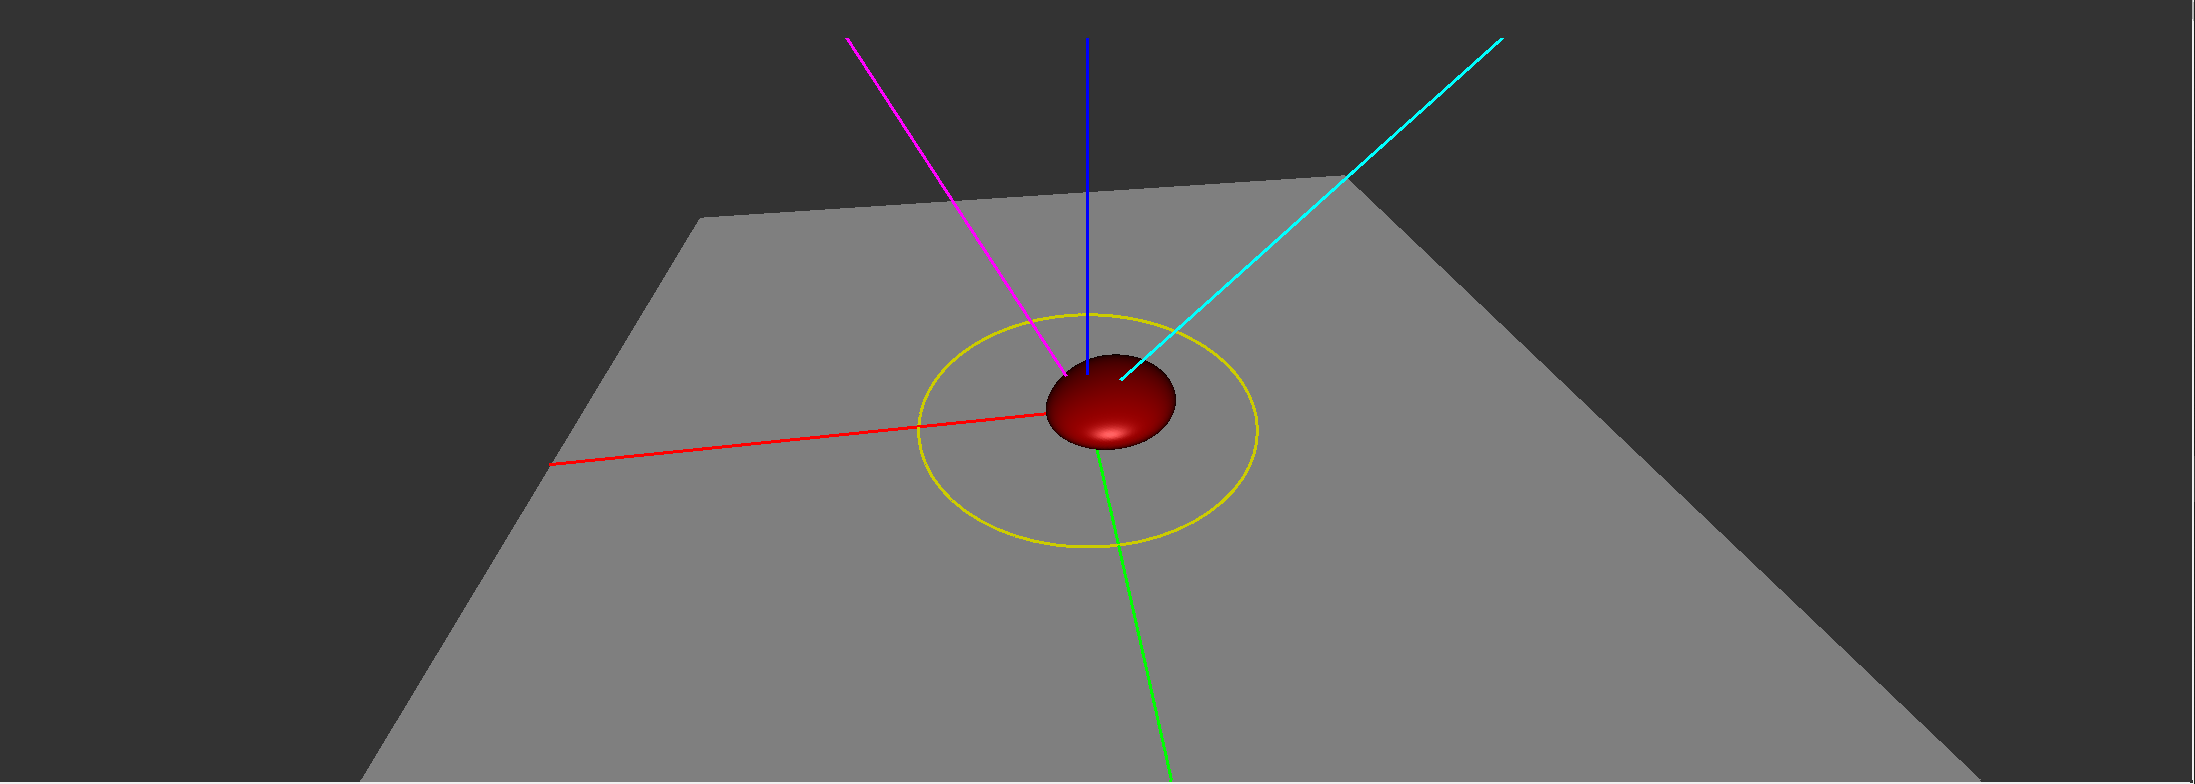
\includegraphics[width=\linewidth]{./Imagens/brdfs/duer-3D-plot}
    % \vspace{0.1px}
    \legend{ \small (a) 3D \textit{plot}}
\endminipage\hfill
\minipage{0.48\textwidth}
  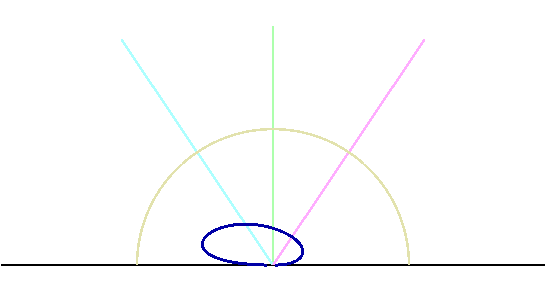
\includegraphics[width=\linewidth]{./Imagens/brdfs/duer-polar-plot.png}
    \legend{ \small (b) \textit{Polar plot}}
\endminipage\hfill
\end{figure}

\begin{figure}[H]
    \caption{\small{Objetos 3D renderizados por este experimento}}\label{fig-duer-eqlang}
\minipage{0.32\textwidth}
  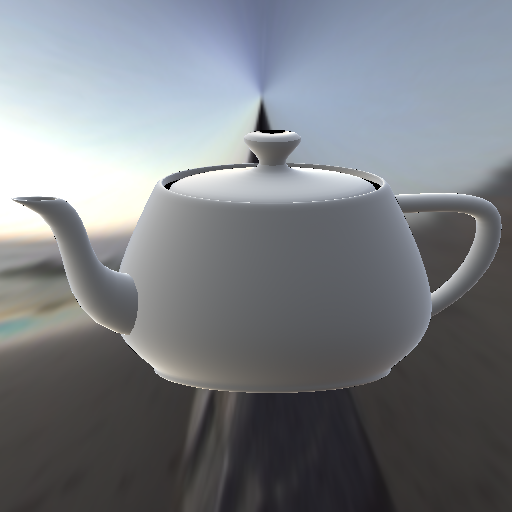
\includegraphics[width=\linewidth]{./Imagens/brdfs/duer-teapot.png}
    \legend{ \small (a) \textit{Teapot}}
\endminipage\hfill
\minipage{0.32\textwidth}
  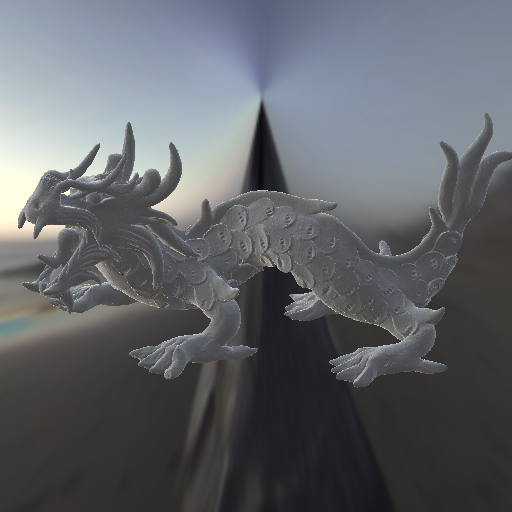
\includegraphics[width=\linewidth]{./Imagens/brdfs/duer-dragon.png}
    \legend{ \small (b) Dragão de Stanford}
\endminipage\hfill
\minipage{0.32\textwidth}%
  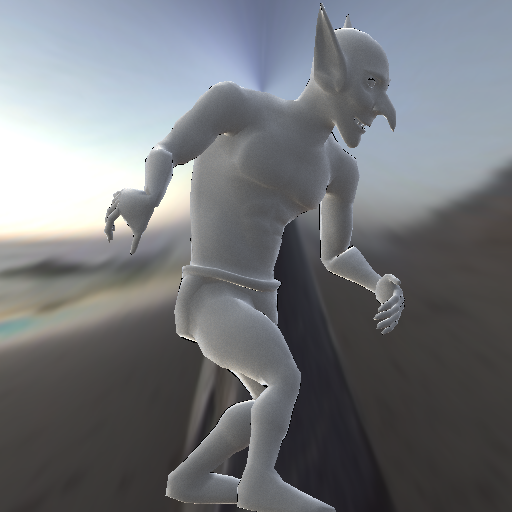
\includegraphics[width=\linewidth]{./Imagens/brdfs/duer-goblin.png}
    \legend{ \small (c) Goblin}
\endminipage
\end{figure}

%%%%%%%%%%%%%%%%%%%%%%%%%%%%%%%%%%%%%%%%%%%%%%%%%
\subsection{Código GLSL Gerado}
%%%%%%%%%%%%%%%%%%%%%%%%%%%%%%%%%%%%%%%%%%%%%%%%%
\begin{codigo}[H]
    \caption{\small Saida do compilador, código GLSL da BRDF deste experimento (parte 1). }
    \label{cod-duer-eqlang-declarations}
\begin{lstlisting}[language=C, inputencoding=utf8]
\end{lstlisting}
\end{codigo}

\begin{codigo}[H]
    \caption{\small Saida do compilador, código GLSL da BRDF deste experimento  (parte 2). }
    \label{cod-duer-eqlang}
\begin{lstlisting}[language=C, inputencoding=utf8]
\end{lstlisting}
\end{codigo}

%%%%%%%%%%%%%%%%%%%%%%%%%%%%%%%%%%%%%%%%%%%%%%%%%
\subsection{Código Fonte em \texttt{EquationLang}}
%%%%%%%%%%%%%%%%%%%%%%%%%%%%%%%%%%%%%%%%%%%%%%%%%
\begin{codigo}[H]
    \caption{\small Código fonte da BRDF deste experimento (parte 1).}
    \label{cod-duer-eqlang}
\begin{lstlisting}[language=tex, frame=none, inputencoding=utf8]
\end{lstlisting}
\end{codigo}
